\chapter{Wazuh UI}
\section{Startseite}
Auf der Startseite sieht man alle aktiven und inaktiven Computer, die mit dem Wazuh Manager verbunden sind.
Von hier aus hat man Schnellzugriff auf alle ``Module'', die Wazuh anbietet.\\

Alle Module und Einstellungen findet man auch im Menü, welches sich durch klicken vom Wazuh Logo öffnen lässt.
\begin{figure}[H]
    \centering
    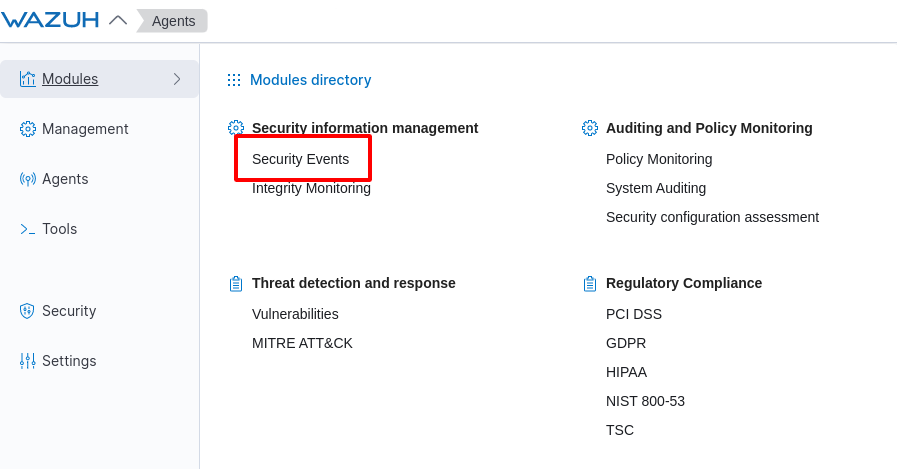
\includegraphics[width=\linewidth]{../img/wazuh-menu.png}
    \caption{Wazuh Menü}
\end{figure}

\section{Security Events}
Die Security Events findet man unter \textbf{Wazuh $\rightarrow$ Modules $\rightarrow$ Security Events}.
Im Modul Security Events werden alle Alerts angezeigt, welche durch die definierten Regeln ausgelöst werden.

\begin{figure}[H]
    \centering
    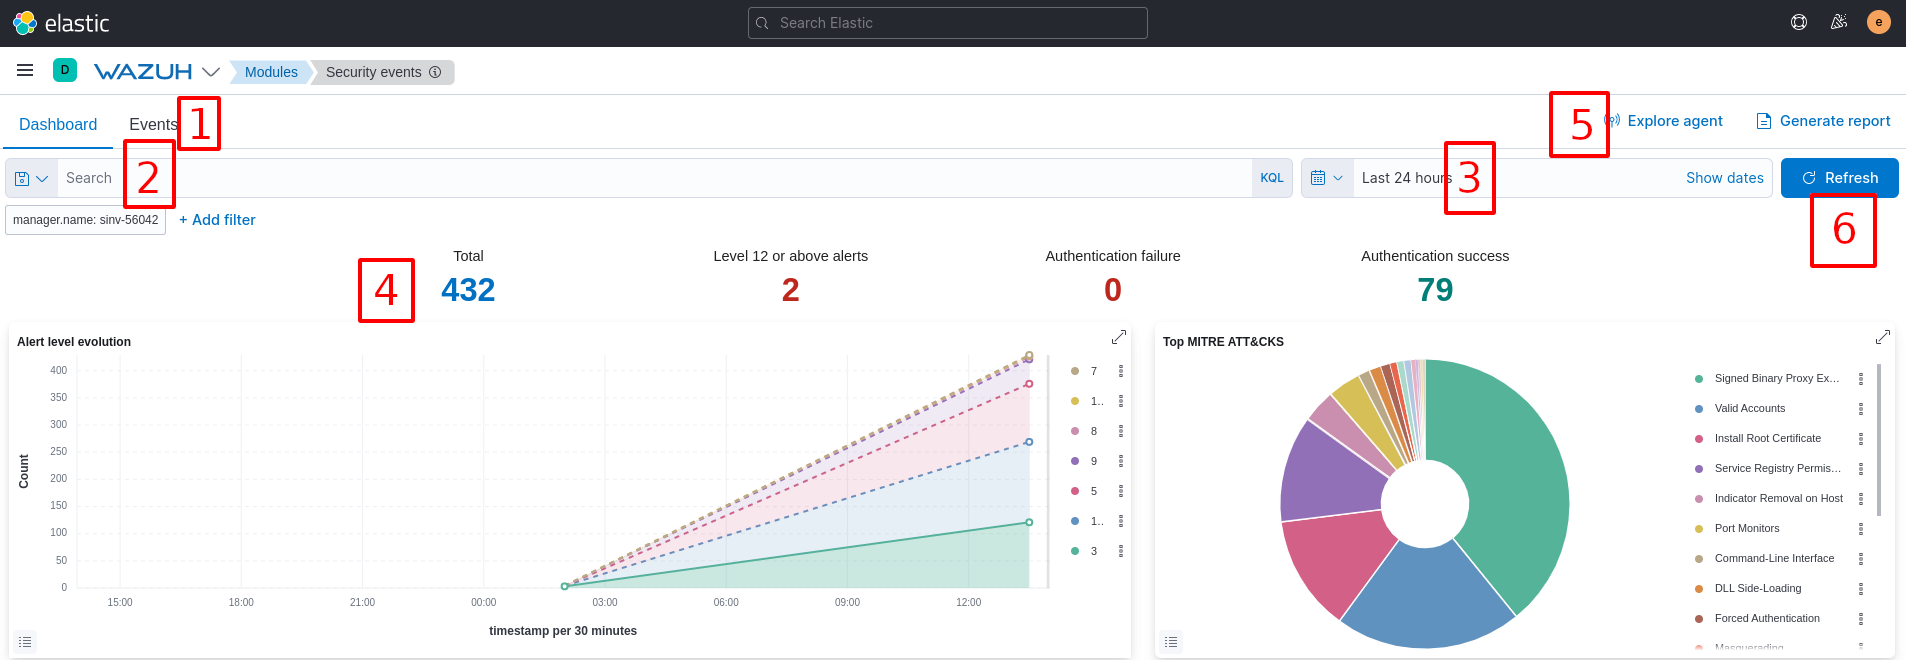
\includegraphics[width=\linewidth]{../img/wazuh-se-1.png}
    \caption{Security Events}
\end{figure}

\begin{enumerate}
    \item Hier kann man zwischen dem Dashboard und den Events wechseln. Das Dashboard zeigt die Alerts und zusammenfassende Diagramme an. Unter Events sieht man nur die Alerts, dafür aber zusätzlich bessere Filter.
    \item In diesem Eingabefeld kann man die Alerts durchsuchen. Mithilfe von Filtern kann man zum Beispiel gewisse Alerts ausblenden oder nur gewisse Anzeigen lassen.
    \item Hier kann man die Zeitspanne angeben, wie lange Zurück man die Alerts ansehen möchte.
    \item Diese Übersicht zeigt an, wie viele Alerts in der eingestellten Zeitspanne generiert wurden und wieviele davon über Level 12 (Kritisch) sind, wieviele davon erfolgreiche Logins und wieviele fehlgeschlagene Logins. Ausserdem zeigt es noch zusammenfassende Diagramme an.
    \item Bei ``Explore Agent'' kann man einen Agent auswählen um nur dessen Alerts anzuzeigen.
    \item Mit ``Refresh'' kann man die neusten Alerts laden.
\end{enumerate}

\begin{figure}[H]
    \centering
    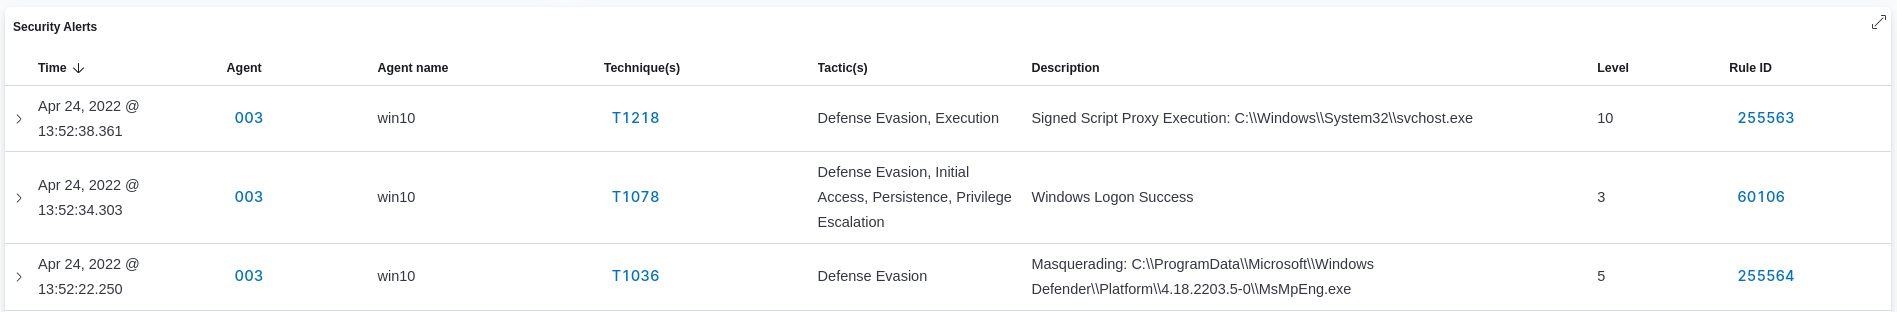
\includegraphics[width=\linewidth]{../img/wazuh-se-2.png}
    \caption{Security Events}
\end{figure}

Hier findet man auch die Alerts. 
In der Liste werden die Alerts angeziegt. 
Diese können nach Titel sortiert werden. 
\begin{itemize}
    \item \textbf{Time} zeigt die Zeit, wann der Alert eingegenen ist.
    \item \textbf{Agent} zeigt von welchem Agent der Alert eingegenen ist.
    \item \textbf{Agent name} zeigt den Computer-Namen des Agent.
    \item \textbf{Technique \& Tatic} zeigt die Mitre Attack Framework Technik an, welcher dieser Alert sein könnte.
    \item \textbf{Description} zeigt eine Beschreibung, um was es sich bei diesem Alert handelt.
    \item \textbf{Level} zeigt das Level des Alerts an. 
    \item \textbf{Rule ID} zeigt an, welche Regel diesen Alert generiert hat.
\end{itemize}

\section{Integrity Monitoring}
Das Integrity Monitoring findet man unter \textbf{Wazuh $\rightarrow$ Modules $\rightarrow$ Integrity Monitoring}.
Im Inventory Monitoring werden alle veränderten Systemdatei und Registry Einträge geloggt. 
Damit kann man bei einem Sicherheitsvorfall eventuell nachvollziehen, wie vorgegangen wurde.

\begin{figure}[H]
    \centering
    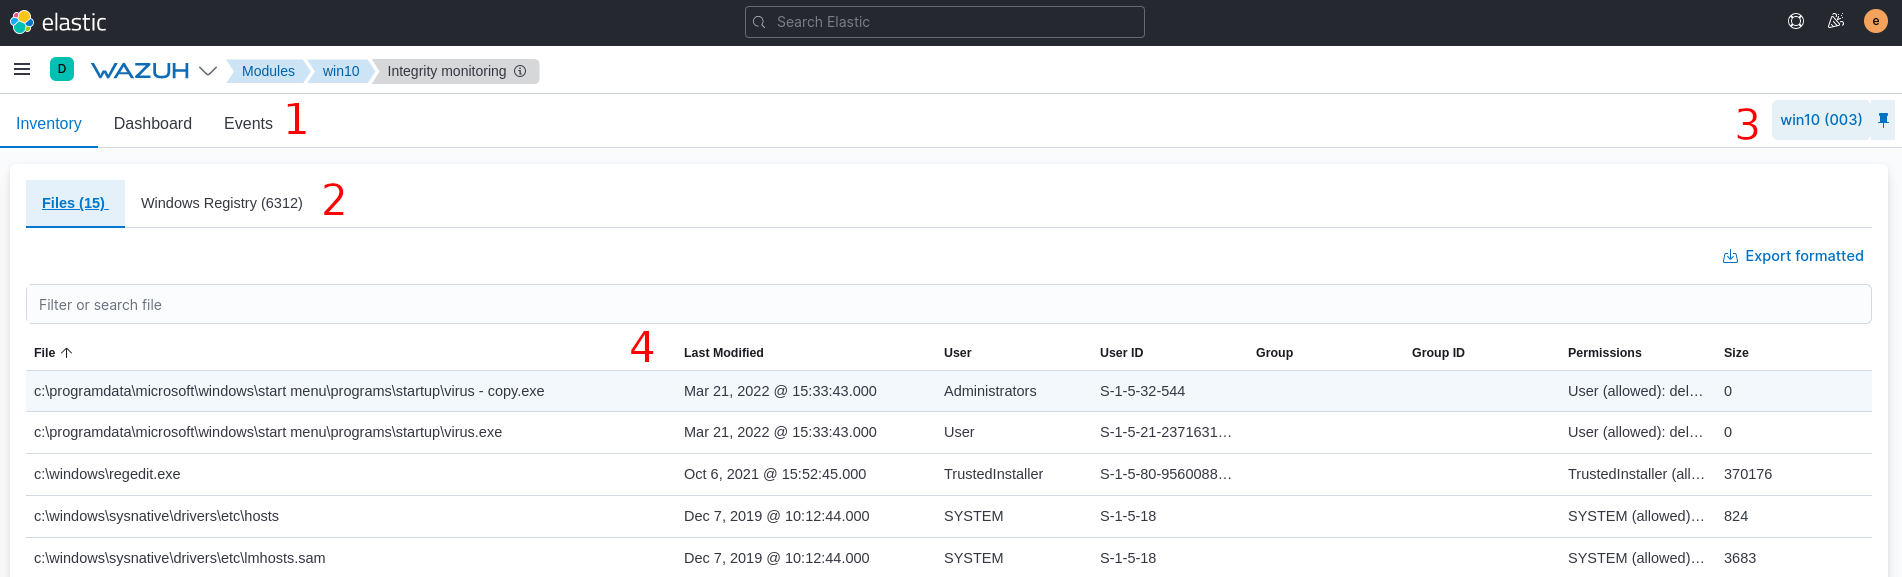
\includegraphics[width=\linewidth]{../img/wazuh-im-inventory.png}
    \caption{Inventory Monitoring}
\end{figure}

\begin{enumerate}
    \item Hier kann man zwischen dem Inventory, dem Dashboard und den Events wechsel.
    \textbf{Inventory} zeigt die veränderten Systemdateien und Registry Einträge an. Im \textbf{Dashboard} findet man zusammenfassende Diagramme und unter \textbf{Events} werden auch alle Änderungen angezeigt, aber zusätzlichen mit einer Unterstützenden Suche. 
    \item Hier kann man zwischen den geänderten Systemdateien und Registry Einträgen wechseln.
    \item Hier kann man den Agent einstellen, welcher man anschauen möchte.
    \item Hier sieht man die Liste von bearbeiteten Systemdateien oder Registry Einträgen.
\end{enumerate}

\section{Rules}
Das Rules findet man unter \textbf{Wazuh $\rightarrow$ Management $\rightarrow$ Rules}.
Hier kann man alle Regeln anschauen und eigene Regeln hinzufügen. 

\begin{figure}[H]
    \centering
    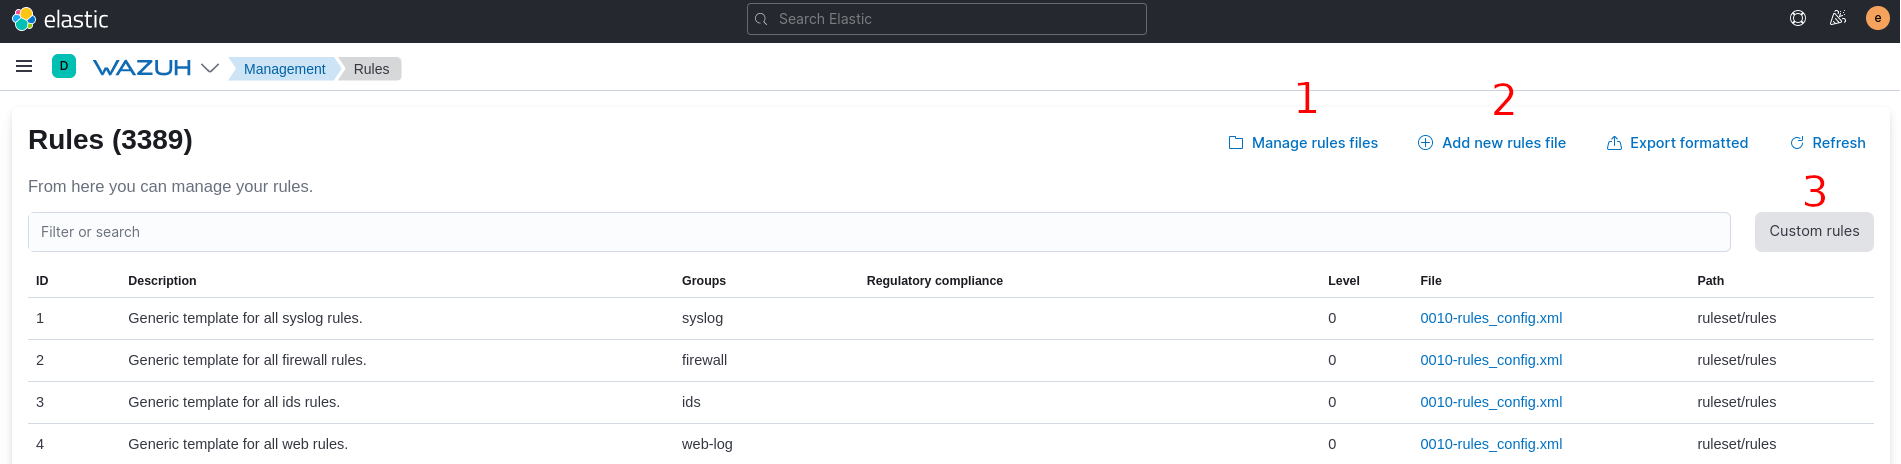
\includegraphics[width=\linewidth]{../img/wazuh-rules.png}
    \caption{Rules}
\end{figure}

\begin{enumerate}
    \item Mit ``Manage rules files'' kann man alle Dateien, welche die Regeln beinhalten, anschauen. 
    \item Mit ``Add new rules file'' kann man eine neue Datei hinzufügen, um neue Regeln zu definieren.
    \item Mit ``Custom rules'' kann man nur die eigenen Regeln oder Regeldateien anzeigen lassen. Alle Regeln von Wazuh werden ausgeblendet.
\end{enumerate}

